\documentclass[twoside,twocolumn]{article}

\usepackage{blindtext} 
\usepackage{graphicx}
\usepackage[sc]{mathpazo} 
\usepackage[T1]{fontenc} 
\linespread{1.05} 
\usepackage{microtype} 


\usepackage[english]{babel} 


\usepackage[hmarginratio=1:1,top=32mm,columnsep=20pt]{geometry} 
\usepackage[hang, small,labelfont=bf,up,textfont=it,up]{caption} 
\usepackage{booktabs} 


\usepackage{lettrine} 


\usepackage{enumitem} 
\setlist[itemize]{noitemsep} 


\usepackage{abstract} 
\renewcommand{\abstractnamefont}{\normalfont\bfseries} 
\renewcommand{\abstracttextfont}{\normalfont\small\itshape} 


\usepackage{titlesec} 
\renewcommand\thesection{\Roman{section}} % 
\renewcommand\thesubsection{\roman{subsection}} 
\titleformat{\section}[block]{\large\scshape\centering}{\thesection.}{1em}{} 
\titleformat{\subsection}[block]{\large}{\thesubsection.}{1em}{} 


\usepackage{fancyhdr} 
\pagestyle{fancy} 
\fancyhead{} 
\fancyfoot{} 
\fancyhead[C]{Bussines Inteligence and Bussines Analytics $\bullet$ Mayo 2020 $\bullet$ } 
\fancyfoot[RO,LE]{\thepage} 


\usepackage{titling} 


\usepackage{hyperref} 


%----------------------------------------------------------------------------------------
%	TILULOS
%----------------------------------------------------------------------------------------


\setlength{\droptitle}{-4\baselineskip} 

\pretitle{\begin{center}\Huge\bfseries} 
\posttitle{\end{center}} 
\title{Business Intelligence and Business Analytics} 
\author{Franklin Carlos Huichi Contreras, Jose Edilberto Pastor Mendoza, \\
Sigfredo Aponte Roldán, Jesus Enrique Sandoval Blas. }
\date{\today} 
\renewcommand{\maketitlehookd}{
\begin{abstract}
\noindent 
Actualmente las tecnologias avanzan y los negocios no se pueden quedar atras, es por ello que las empresas tienen que estar en sintonia con las nuevas estrategias del mercado para poder evolucionar. Es por ello que la utilizacion de Business Inteligence y Business Analytics cada vez se esta haciendo nesecario e imprecindible para cada negocio, esto debido que se le da un valor agregado a la informacion brindada por los datos, Businnes Inteligence centrandose en el pasado para generar reportes del presente revisando las tendencias de cada periodo que esta tomando como rumbo nuestra empresa y Businnes Analytics centrandose en el presente para poder tomar desiciones para el futuro intentando analizar como evolucionara los negocios para poder reaccionar ante ello y generar mas redito de ello. Ambas estrategias de negocios se basan en la recopilacion de datos de una empresa para convertirlos en informacion y usarla para los analisis, asimismo mostrar graficos estadisticas para el mejor aprovechamiento de la informacion y asi tomar las mejores decisiones de negocios.
\end{abstract}
\begin{abstract}
\noindent 
Currently technologies advance and business cannot be left behind, that is why companies have to be in tune with new market strategies in order to evolve. That is why the use of Business Intelligence and Business Analytics is becoming nesecarious and essential for each business, this is because an added value is given to the information provided by the data, Businnes Intelligence focusing on the past to inform reports of the present reviewing the trends of each period that our company is taking as a direction and Businnes Analytics focuses on the present to be able to make decisions for the future trying to analyze how businesses will evolve to be able to react to it and generate more profit from it. Both business strategies are based on the collection of data from a company to convert it into information and use it for analysis, show statistical graphics for the best use of information and thus make the best business decisions.

\end{abstract}
}

%----------------------------------------------------------------------------------------

\begin{document}

% Print the title
\maketitle

%----------------------------------------------------------------------------------------
%	INTRODUCCION
%----------------------------------------------------------------------------------------

\section{Introduccion}
\lettrine[nindent=0em,lines=3]{L}a actual sociedad del conocimiento cuenta con una gran cantidad de datos e información en múltiples formatos o estilos (Big Data) que fácilmente sobrepasan la capacidad de procesamiento humana. Su producción es exponencial y continua, lo que nos ha llevado a desarrollar nuevos recursos y tecnologías para almacenar, procesar, recuperar y sacar provecho de toda esta información. En el sector empresarial se ha venido desarrollado un campo conocido como Business Intelligence (BI) o inteligencia de negocios con el objetivo de recopilar, analizar y diseminar la información para el beneficio de los negocios y la toma de decisiones
lo cual ha permitido a muchas industrias generar inteligencia, o mejor, derivar información y conocimiento como un instrumento para
mejorar la ventaja competitiva.  No obstante, la BI adquiere la connotación de Learning Analytics (LA) o analítica de datos, que trata también con la medición, recopilación, análisis e informes de datos y sus contextos, con el fin de comprender y optimizar las tareas de una empresa, lo cual desde la BI, corresponde a mejorar la ventaja competitiva en una organización.

%----------------------------------------------------------------------------------------
%	Objetivos
%----------------------------------------------------------------------------------------


\section{Marco teorico}

\begin{itemize}
\item Inteligencia de Negocios (BI): \\ 
La inteligencia de negocios es el proceso de recopilar, almacenar y analizar datos de operaciones empresariales. La inteligencia de negocios ofrece metricas integrales de negocio,
en tiempo real con el fin de poder mejorar la toma de decisiones. Con una mejor inteligencia de negocio podemos crear valores de referencia de rendimiento, detectar tendencia del mercado,
aumentar el cumplimiento y mejorar en todos los aspectos de la empresa.
\begin{center}
	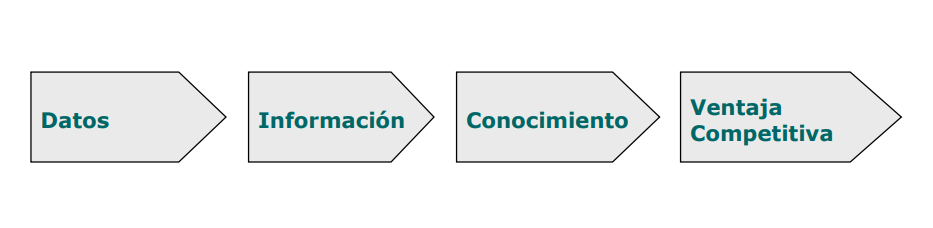
\includegraphics[width=7cm]{./Imagenes/bi} 
\end{center}

\item Analisis de Negocio (BA): \\ 
El análisis de negocio es el conjunto de métodos y técnicas utilizadas para trabajar como enlace entre los stakeholders con el fin de comprender la estructura, políticas y operaciones de una organización y recomendar soluciones que permitan alcanzar sus objetivos. El análisis de negocio implica la comprensión de cómo funcionan las organizaciones para llevar a cabo sus propósitos y la definición de las capacidades que requiere para proporcionar productos y servicios a los grupos de interés externos.

\end{itemize}



%----------------------------------------------------------------------------------------
%	DESARROLLO
%----------------------------------------------------------------------------------------

\section{Desarrollo}

\subsection{¿Que no es Business Intelligence?}
Comencemos con los que no es BI. BI no es:
Un solo producto. Aunque muchos productos excelentes pueden ayudarlo a implementar BI, BI no es un producto que se pueda comprar e instalar para resolver todos sus problemas "desde el primer momento". BI tampoco es una tecnologia, aunque las herramientas y tecnologías de DW, como las herramientas ETL de bases de datos relacionales, las herramientas de interfaz de usuario de BI y los servidores, se usan típicamente para admitir aplicaciones de BI. BI no es solamente una tecnologia.

\subsection{Si eso es lo que BI no es, ¿Entonces qué es?}
BI combina productos, tecnología y métodos para organizar la información clave que la gerencia necesita para mejorar las ganancias y el rendimiento. En términos más generales, pensamos en bi como información comercial y análisis de negocios dentro del contexto de procesos comerciales clave que conducen a decisiones y acciones, Que resultan en un mejor desempeño comercial, en particular BI significa apalancar los activos de información dentro de los procesos comerciales clave para lograr un mejor rendimiento comercial. Incluye información y análisis de negocios que son:

\begin{itemize}	
	\item Utilizado dentro de un contexto de procesos comerciales clave.
	\item Apoyar decisiones y acciones.
	\item Conducir a un mejor rendimiento empresarial.

\end{itemize} 

\subsection{¿Que es Business Analytics}

Business analytics es un campo que impulsa cambios prácticos basados en datos en una empresa. Es una aplicación práctica de análisis estadístico que se centra en proporcionar recomendaciones viables. Los analistas en este campo se centran en cómo aplicar los conocimientos que derivan de los datos. Su objetivo es sacar conclusiones concretas sobre un negocio respondiendo preguntas específicas sobre por qué sucedieron las cosas, qué sucederá y qué se debe hacer.
 
El análisis cuando se aplica a los datos, crea información. en su forma más amplia, abarca una amplia gama de disciplinas, incluidas la inteligencia empresarial, las estadísticas, la gestión de datos y la ciencia de datos. Por ejemplo, el análisis avanzado y el aprendizaje automático es un subconjunto de análisis que se enfoca en extraer una mayor comprensión a través de técnicas matemáticas. A menudo trata de entender por qué suceden las cosas y predecir lo que sucederá en lugar de simplemente resumir lo que ya sucedió. una vez creado, se necesita actuar sobre la información para crear valor. donde el análisis crea información, BA se preocupa por tomar esa información y usarla para crear valor.

\begin{center}
	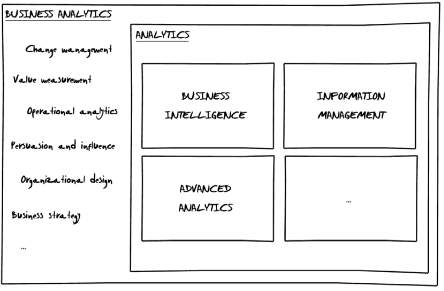
\includegraphics[width=7cm]{./Imagenes/ba} 
\end{center}

\subsection{¿En que se diferencian Business Intelligence con Business Analytics?}
\begin{itemize}	
	\item La diferencia principal en ambas ideas es que el Business Inteligence se enfoca en los datos que manejamos los datos ya recopilados la cual la podemos convertir en informacion y usarla para analizarlas y entender el pasado del negocio. Por otro lado el Business Analytics nos permitira centrarnos en el presente para crear una vision clara del futuro y predecir (mediante modelos predectivos) para adelantarnos al futuro.
	\item La  diferencia entre los dos radica en comprender el valor de la percepción y convencer a una organización para que cambie la forma en que hace negocios.
\end{itemize} 





\subsection{¿En que se asemejan Business Intelligence con Business Analytics?}
Business Intelligence y Business Analytics se basan en la recopilacion de datos de una empresa para convertirlos en informacion y usarla para los analisis, asimismo mostrar graficos estadisticas para el mejor aprovechamiento de la informacion y asi tomar las mejores decisiones de negocios.










\subsection{¿Que es Analisis de Negocios ,BA?}
El análisis de negocio es el conjunto de métodos y técnicas utilizadas para trabajar como enlace entre los stakeholders con el fin de comprender la estructura, políticas y operaciones de una organización y recomendar soluciones que permitan alcanzar sus objetivos.

El análisis de negocio implica la comprensión de cómo funcionan las organizaciones para llevar a cabo sus propósitos y la definición de las capacidades que requiere para proporcionar productos y servicios a los grupos de interés externos. Incluye la definición de los objetivos de la organización, cómo esos objetivos se conectan a objetivos específicos, que determinan las líneas de acción que una organización tiene que realizar para alcanzarlos, y definir cómo interactúa las distintas unidades de la empresa y las partes interesadas dentro y fuera de ella.

El análisis de negocio consiste en entenderlo y saber sus procesos, proponer alternativas de solución y definir el alcance de la solución seleccionada considerando todos los recursos de la organización. Esto se debe a que los procesos de negocio constituyen el pilar fundamental de la operación de toda organización privada o pública, por lo que su identificación y categorización sin ambigüedades, comprensión funcional de su estructura básica, análisis y rediseño, y administración eficaz de su desempeño son de la mayor relevancia para incrementar la competitividad de las empresas.


\begin{center}
	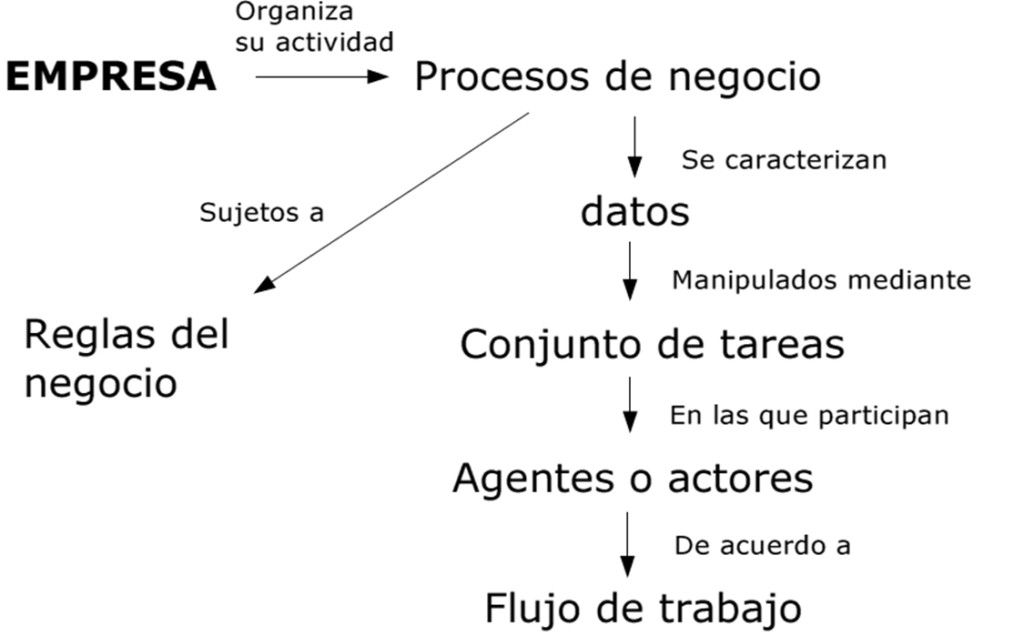
\includegraphics[width=7cm]{./Imagenes/AnalisisNegocio} 
\end{center}


\subsection{Ejemplos de análisis de negocios}

\begin{itemize}	
	\item Las técnicas de análisis de negocios se dividen en dos áreas principales. La primera es la inteligencia de negocios básica. Esto implica examinar datos históricos para tener una idea de cómo se desempeñó un departamento de negocios, un equipo o un miembro del personal durante un tiempo determinado. Esta es una práctica madura de la que la mayoría de las empresas obtienen un buen desempeño.
	\item La segunda área de análisis de negocios implica un análisis estadístico más profundo. Esto puede significar hacer análisis predictivos aplicando algoritmos estadísticos a datos históricos para hacer una predicción sobre el rendimiento futuro de un producto, servicio o cambio en el diseño del sitio web. O podría significar el uso de otras técnicas analíticas avanzadas, como el análisis de clústeres para agrupar a los clientes según las similitudes en varios puntos de datos. Esto puede ser útil en campañas de marketing dirigidas.
\end{itemize} 

Los tipos específicos de análisis de negocios incluyen:
\begin{itemize}	
	\item Análisis descriptivo, que realiza un seguimiento de los indicadores clave de rendimiento para comprender el estado actual de una empresa.
	\item Análisis predictivo, que analiza los datos de tendencias para evaluar la probabilidad de resultados futuros.
	\item Análisis prescriptivo, que utiliza el rendimiento pasado para generar recomendaciones sobre cómo manejar situaciones similares en el futuro.
\end{itemize} 


Si bien los dos componentes del análisis de negocios (inteligencia empresarial y análisis avanzado) a veces se usan indistintamente, existen algunas diferencias clave entre estas dos técnicas de análisis de negocios. Por ejemplo, la inteligencia de negocios responde a las preguntas: ¿Qué sucedió? ¿Cuándo? ¿Quién lo hizo? ¿Con qué frecuencia? Mientras que la analítica avanzada, por su parte, responde cuestionamientos como: ¿Por qué sucedió? ¿Volverá a suceder? ¿Qué pasará si modificamos el factor X? ¿Qué más nos dicen los datos que tal vez nunca se nos habría ocurrido preguntar?.








%----------------------------------------------------------------------------------------
%	CONCLUSIONES
%----------------------------------------------------------------------------------------


\section{Conclusiones}
\begin{itemize}	
	\item En conclusion tanto Business Analytic y Business Inteligence tienen mas diferencias que semejanzas debido que a pesar de que cada uno recopilan datos y lo convierten en
informacion cada uno tiene un mundo diferente despues de partir de esa premisa ya que uno analiza el pasado para plasmarlo al presente y el otro analiza lo que va a ocurrir en un futuro proximo para poder tomar mejores decisiones.

\end{itemize} 



%----------------------------------------------------------------------------------------
%	BIBLIOGRAFIA
%----------------------------------------------------------------------------------------


\begin{thebibliography}{99} 

\bibitem[Silvia Chavez y Carmen Contreras, 2018]{}
\newblock Implementación de Business Intelligence, para el proceso de toma de decisiones del área de ventas.

\bibitem[Hans Peter Luhn 1958]{}
\newblock A Business Intelligence System

\bibitem[Alex Rayón, 2015]{Universidad de Deusto}
Conceptos básicos del Business Intelligence.

\bibitem[Jordi Conesa y Josep Curto, 2010]{}
\newblock Introduccion al Business Intelligence

\bibitem[Margaret Rouse, 2019]{}
\newblock Análisis de negocios (BA)

\bibitem[Noodle Editorial Staff, 2018]{}
\newblock Business analytics career paths

\bibitem[Josep Lluis Cano, 2007]{}
\newblock Business Intelligence: competir con información


\bibitem[Curto J., 2010]{} 
\newblock Introducción al Business Intelligence. Editorial UOC.

\bibitem[Kimball R. and Ross M., 2002]{} 
\newblock  The Data Warehouse Toolkit: The Complete Guide to Dimensional Modeling. Wiley

\bibitem[Carolina A., 2017]{} 
\newblock  Análisis de Negocio (Business Analysis, BA)

\bibitem[Dr. Jorge Alexander AristizabalF., 2019]{} 
\newblock  Business Intelligence and Learning Analytics as Integrated Systems for School Management
 
\end{thebibliography}


%----------------------------------------------------------------------------------------


\end{document}
